\section{Multi-scale Local Binary Pattern}
In questo capitolo verranno presentati alcuni concetti teorici e gli stumenti utilizzati per lo sviluppo dell'applicazione. Il primo paragrafo introdurrà il descrittore di feature \acf{LBP}. Verrà analizzata una sua variante, ovvero Uniform \acs{LBP}, che viene utilizzato per ridurre la lunghezza del vettore di feature. Analizzeremo infine la sua estensione \acf{MLBP}.

\subsection{Local Binary Pattern}

\acf{LBP} è un efficiente texture operator, introdotto per la prima volta nel 1994 \cite{LBPfirst}. Le feature estratte con questo metodo vengono utilizzate per la classificazione di immagini in ambito della computer vision.
\acs{LBP} associa ai pixel dell'immagine un'etichetta, determinata tramite un'operazione di confronto tra il pixel in esame ed un certo numero di pixel nelle sue vicinanze, \emph{neighborhood}.
Tra le caratteristiche principali di \acs{LBP} troviamo:

\begin{itemize}
	\item è robusto alla variazione uniforme dell'illuminazione dell'immagine;
	\item è robusto al rumore;
	\item non è invariante alle rotazioni dell'immagine;
	\item non è invariante alla scala.
\end{itemize}

Un altra importante proprietà è infine la sua semplicità computazionale che lo rende ideale per l'analisi delle immagine in \acf{RT}.

\subsubsection{Descrizione}

L'idea alla base dell'operatore \acf{LBP} è che le texture bidimensionali possono essere descritte attraverso pattern locali.
L'implementazione base dell'operatore \acs{LBP} etichetta i pixel dell'immagine attraverso un'operazione di sogliatura dei pixel contenuti in una maschera 3 x 3.

 Il pixel centrale viene confrontato con ogni vicino ed il risultato del confronto viene espresso con un numero binario.\\

\begin{figure}[ht]
\begin{center}
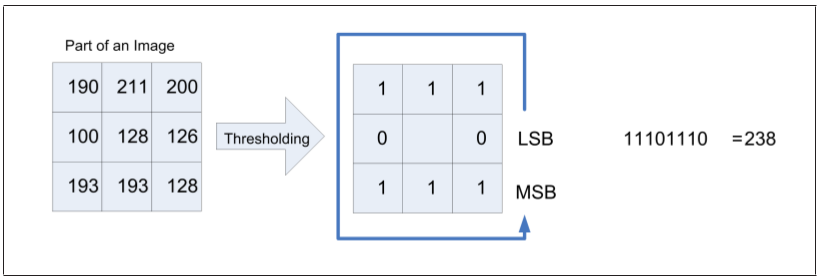
\includegraphics[width=.95\textwidth]{img/LBP_code}
\caption{ Estrazione del codice LBP.}
\label{fig:LBPcode}
\end{center}
\end{figure}

Riferendoci alla figura \ref{fig:LBPcode} il processo di etichettatura dei pixel è il seguente. Il livello di grigio del pixel centrale, detto anche \emph{pivot} viene confrontato con il livello di grigio di tutti gli altri pixel della maschera che viene binarizzata attraverso la seguente funzione:

\begin{equation}
s(x) = 	\begin{cases} 1, & \mbox{se } x \ge 0 \\ 0, & \mbox{se } x < 0 \end{cases}
\end{equation}

dove $x$ è la differenza tra l'intensità del livello di grigio di un pixel del \emph{neighborhood} ed il livello di grigio del pixel pivot. I valori così ottenuti vengono concatenati in senso antiorario andando a formare un codice binario di 8 bit la cui conversione decimale rappresenta il codice \acs{LBP} del pixel pivot.

\subsubsection*{Descrittore}
Il numero totale di codici \acs{LBP} è pari a $2^8 = 256$.
L'istogramma dei codici LBP calcolati sui pixel dell'immagine può essere utilizzato come descrittore della texture. In figura \ref{fig:istCompleteLBP} è mostrato l'istogramma di un immagine LBP.

\begin{figure}[ht]
\begin{center}
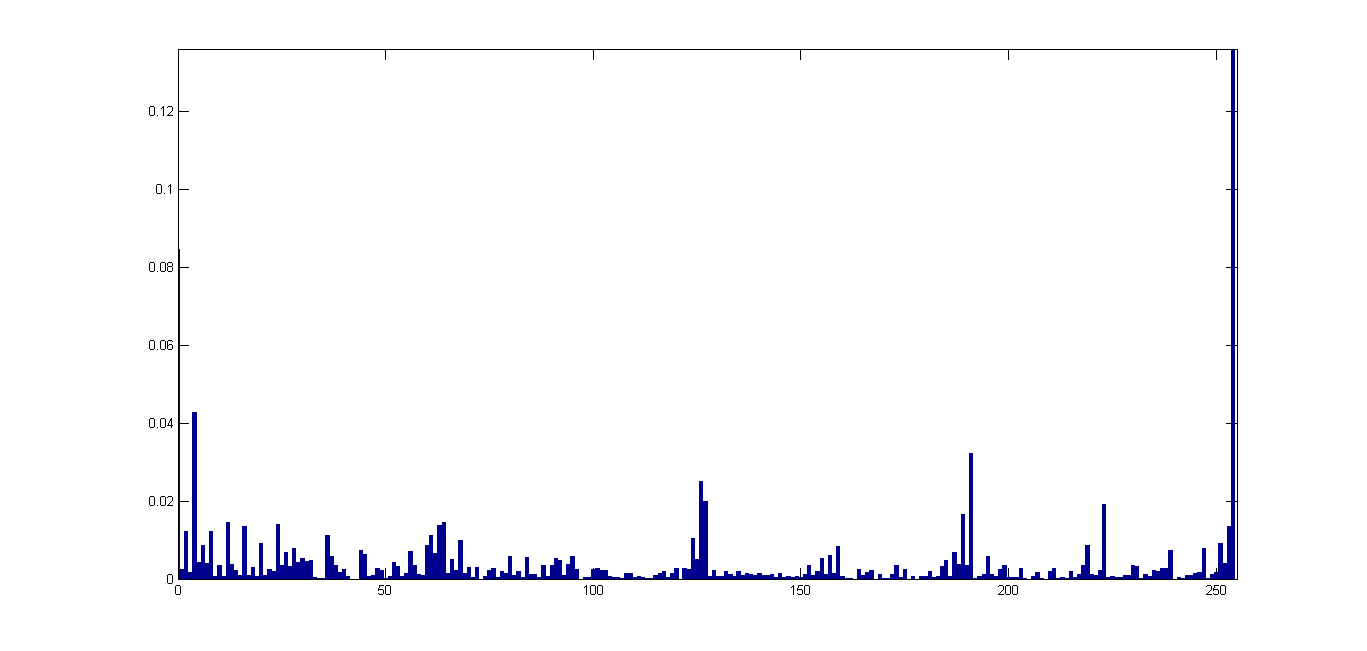
\includegraphics[width=.95\textwidth]{img/hist-complete}
\caption{ Istogramma normalizzato di un'immagine LBP. }
\label{fig:istCompleteLBP}
\end{center}
\end{figure}

Per il calcolo dell'istogramma si utilizza la seguente formula:

\begin{equation}
h(i) = \sum_{x,y} B(LBP_{P,R}(x, y)) = i, i \in  [0, 2^P-1 ]
\end{equation}

dove

\begin{equation}
B(v) = 	\begin{cases} 1, & \mbox{v = true} \\ 0, & \mbox{altrimenti} \end{cases}
\end{equation}

\subsection{Extended LBP}
\label{MLBP:extended}
Finora abbiamo considerato come neighborhood i pixel adiacenti a quello di pivot. Una variante dell'operatore \acs{LBP} è l' \acf{ELBP} o \acf{CLBP} . \acs{ELBP} considera come neighborhood i $P$ pixel che si trovano ad una distanza $R$ dal pivot. Le coordinate dei $P$ pixel si possono ottenere con la seguente formula:

\begin{equation}
(x_p, y_p) = \left(  - Rsin\left( \frac{2\pi p}{P} \right), Rcos\left( \frac{2\pi p}{P} \right) \right)   , \quad p = 0, \cdots, P-1
\end{equation}

Nel caso in cui le coordinate ottenute non corrispondono alla griglia discreta dell'immagine si effettua una interpolazione bilineare.

In figura \ref{fig:NeighborhoodLBP} sono mostrati alcuni risultati dell'applicazione della formula appena descritta.

\begin{figure}[ht]
\begin{center}
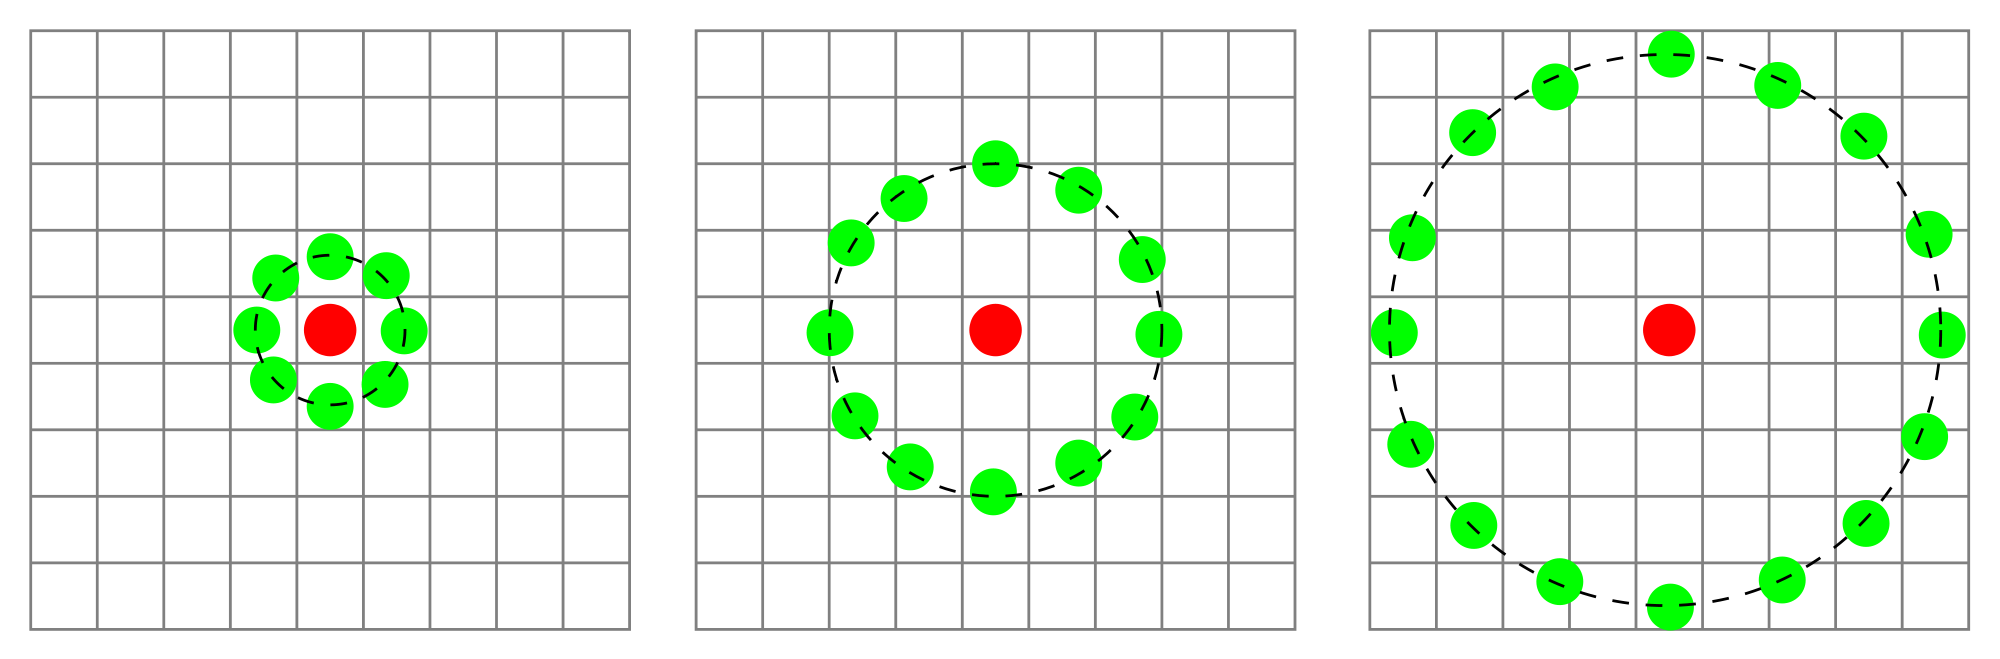
\includegraphics[width=.95\textwidth]{img/raggio_LBP}
\caption{ Neighborhood per il calcolo del codice LBP nei casi: $(P=8, R=1)$, $(P=12, R=2)$ e $(P=16, R=4)$. }
\label{fig:NeighborhoodLBP}
\end{center}
\end{figure}


La formula seguente permette di calcolare, in base dieci, il codice LBP di lunghezza $P$ e raggio $R$ generico di un pixel.

\begin{equation}
LBP_{P,R}(x, y) = \sum_{p=0}^{P-1}{s(g_p - g_c)2^p}
\end{equation}

\subsection{Uniform Local Binary Pattern}
Come accennato precedentemente l'istogramma dell'immagine LBP è utilizzato come descrittore della texture. Utilizzando l'operatore LBP base, otteniamo un istogramma con $256$ classi. Per ridurre la dimensione del descrittore si può utilizzare Uniform \acf{LBP}. Uniform \acs{LBP} considera solo i pattern in cui occorrono al più due transizioni da $0$ a $1$ o da $1$ a $0$ tra pixel adiacenti. Per esempio:

\begin{itemize}
	\item $00000000 \rightarrow 0$ transizioni
	\item $01110000 \rightarrow 2$ transizioni
	\item $11001111 \rightarrow 2$ transizioni
	\item $11001001 \rightarrow 4$ transizioni
	\item $01010010 \rightarrow 6$ transizioni
\end{itemize}

I pattern che soddisfano le condizioni di Uniform \acs{LBP} sono in totale $58$, come mostrato in figura \ref{fig:uniformLBP}.

\begin{figure}[ht]
\begin{center}
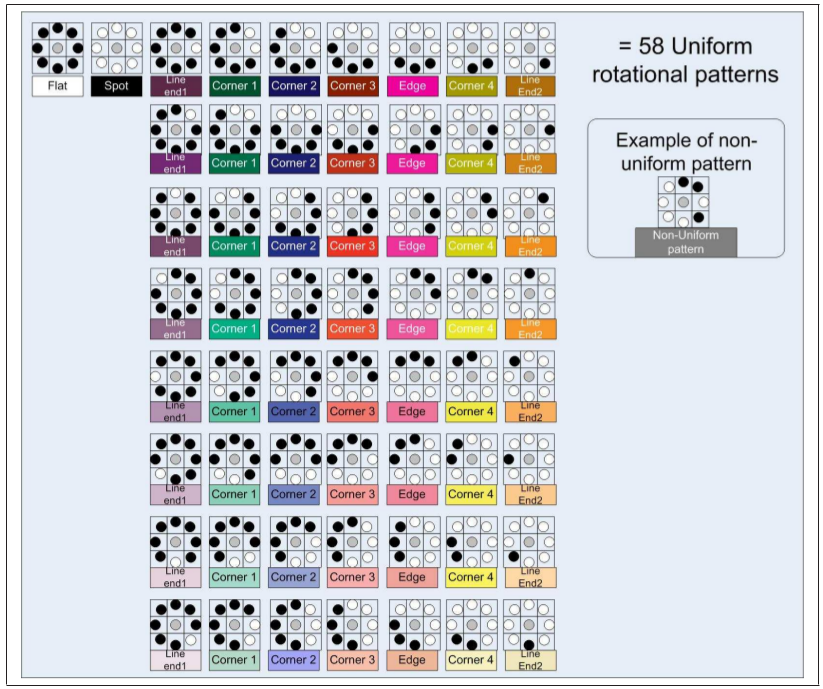
\includegraphics[width=.95\textwidth]{img/uniform_LBP}
\caption{ Pattern di Uniform LBP.}
\label{fig:uniformLBP}
\end{center}
\end{figure}

Questa variante si basa sul fatto che le feature così estratte sono più robuste al rumore e l'istogramma risultante è di dimensione inferiore mantenendo comunque le feature rilevanti.

In figura \ref{fig:istUniformLBP} è mostrato l'istogramma di un immagine su cui è stato applicato l'operatore di Uniform \acs{LBP}.

\begin{figure}[ht]
\begin{center}
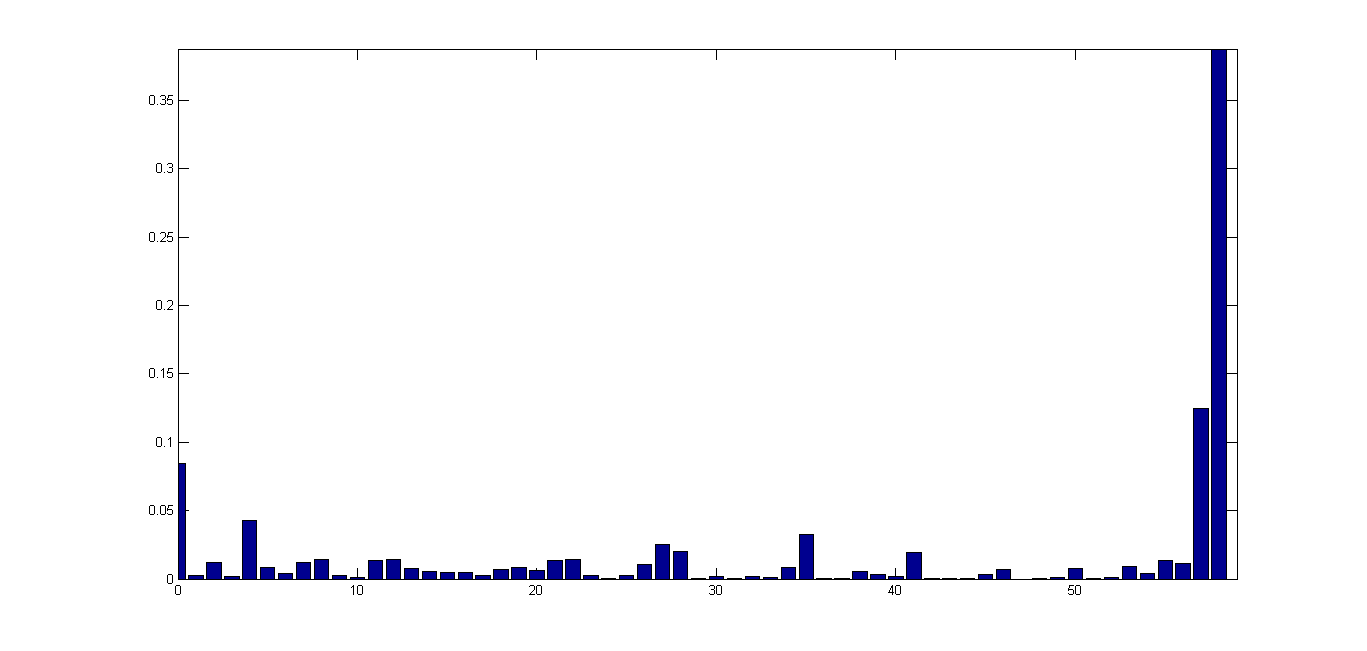
\includegraphics[width=.95\textwidth]{img/hist-uniform}
\caption{ Istogramma normalizzato di una immagine su cui è stato applicato l'operatore di Uniform \acs{LBP}. I primi $58$ pattern sono quelli uniformi, mentre l'ultimo pattern corrisponde a tutti i pixel con codice non uniforme.}
\label{fig:istUniformLBP}
\end{center}
\end{figure}

Per ottenere il codice di Uniform \acs{LBP} si utilizza la formula seguente:

\begin{equation}
LBP_{P,R}^{u2}(x, y)=	
\begin{cases} 
I(LBP_{P,R}(x, y)), & \mbox{se } U(LBP_{P,R}) \le 2, I(z) \in [0, (P-1)P+2 )   \\
(P-1)P+2, & \mbox{altrimenti}
\end{cases}
\end{equation}

dove la funzione $U(x)$ calcola il numero di transizioni.

\begin{equation}
U(LBP_{P,R}) = |s( g_{P-1} - g_{c}) - s(g_{0} - g_{c}) | + \sum_{p = 1}^{P} |s(g_{p} - g_{c}) - s( g_{P-1} - g_{c}) |
\end{equation}

\subsection{Multiscale Local Binary Pattern}
\acf{MLBP} è un'estensione dell'operatore \acs{LBP}. \acs{MLBP} è ottenuto combinando i descrittori delle texture ottenuti facendo variare il raggio $r \in \left\lbrace  r_1, r_2, \cdots, r_R \right\rbrace$ per la determinazione dei neighbor. 
Alternativamente \acs{MLBP} può essere ottenuto applicando l'operatore \acs{LBP} con raggio costante su l'immagine a risoluzione ridotta. Quest'ultimo metodo è meno efficace in quanto riducendo la risoluzione dell'immagine risulta più difficile estrarre informazioni sul contrasto tra piccole regioni lontane fra loro.

Le feature estratte con \acs{MLBP} risultano migliori rispetto a \acs{LBP} per la classificazione di immagini.

\subsubsection{Descrittore}
\label{mlbp:desc-mlbp}
Il descrittore della texture ottenuto con \acs{MLBP} è la concatenazione degli istogrammi ottenuti applicando iterativamente \acs{LBP} sulla stessa immagine al variare del raggio $r \in \left\lbrace  r_1, r_2, \cdots, r_R \right\rbrace$. Il descrittore è dato dalla seguente formula:

\begin{equation}
\label{mlbp:eq-descriptor}
f = [h_{P, r_{1}}, h_{P, r_{2}}, \cdots, h_{P, r_R}]
\end{equation}

\noindent dove

\begin{equation}
h_{P,r}(i) = \sum_{x, y} B(LBP_{P,r}(x, y)) = i, i \in  [0, L-1 ], r \in \left\lbrace  r_1, r_2, \cdots, r_R \right\rbrace
\end{equation}

\noindent con $L$ numero massimo di classi dell'istogramma e

\begin{equation}
B(v) = 	\begin{cases} 1, & \mbox{v = true} \\ 0, & \mbox{altrimenti} \end{cases}
\end{equation}

\subsection{Filtro di smoothing gaussiano}
I filtri di \emph{smoothing} vengono utilizzati principalmente per ridurre il rumore presente nell'immagine. Sono anche detti \emph{filtri di media}. Infatti facendo scorrere lungo l'immagine la maschera del filtro, detta anche \emph{kernel mask}, il valore di ogni pixel viene sostituito con la media pesata dei livelli di grigio dei pixel interni alla regione della maschera. Il processo di smoothing permette di ridurre i dettagli meno significativi dell'immagine e mettere in risalto le caratteristiche strutturali della stessa.
Un effetto indesiderato dello smoothing è quello di produrre un'immagine sfocata, soprattutto se applicato iterativamente.
La figura \ref{fig:kernelMask} mostra un filtro di smoothing generico 3x3. La maschera del filtro verrà moltiplicata per un coefficiente di normalizzazione in modo tale che la somma degli elementi della mascherà sia uno. I coefficienti della maschera vengono scelti secondo il seguente principio: il peso associato al pixel centrale assume un valore superiore rispetto agli altri. I pesi associati agli altri pixel assumono valori decrescenti all'aumentare della distanza dal pixel centrale. In altre parole si vuole fare in modo che il pixel centrale abbia una maggiore importanza nel calcolo della media. Viceversa i pixel più lontani da quello centrale peseranno di meno nel calcolo della media. Questo permette di ridurre l'effetto indesiderato del processo di smoothing.

\begin{figure}[ht]
\begin{center}
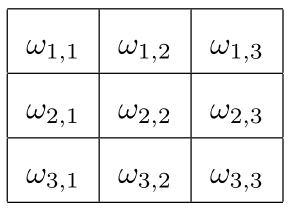
\includegraphics[width=.3\textwidth]{img/kernel_mask}
\caption{ Esempio di una kernel mask di dimensioni 3x3, dove $\omega_{i,j}$ reppresenta il peso applicato al valore del livello di grigio del corrispettivo pixel nell'immagine}
\label{fig:kernelMask}
\end{center}
\end{figure}

I coefficienti della maschera sono calcolati utilizzando la \emph{2D Gaussian Smoothing Operator} $G(x,y)$, cui formula è riportata qui di seguito:

\begin{equation}
G(x, y) = e^{- \frac{(x^2 + y^2)}{2\sigma^2}}
\end{equation}

La dimensione $n$ della kernel mask è legata al valore di $\sigma$ dalla seguente formula:

\begin{equation}
6\sigma - 1 = n
\end{equation}

%\begin{center}
%\begin{tabular}[ht]{|c|c|c|}\hline
%	$\omega_{1,1}$ & $\omega_{1,2}$ & $\omega_{1,3}$ \\ \hline
%	$\omega_{2,1}$ & $\omega_{2,2}$ & $\omega_{2,3}$ \\ \hline
%	$\omega_{3,1}$ & $\omega_{3,2}$ & $\omega_{3,3}$ \\ \hline
%\end{tabular}
%\end{center}